\subsection{Neural Network Architecture}
\label{subsec:net}
Similar to AlphaZero \cite{alphazero}, we use a single neural network with a policy head and value head.
Our first layer is a mixture of a convolutional layer and a dense layer to process the spatial and scalar data into an 8x16 layer with depth 256.
Each filter of the first layer has one additional non-spatial parameter for each scalar input value.
The sum of these scalar values, weighted by their respective parameters, is added to the filter output before the activation function.
This layer is followed by several residual blocks which contain convolutional layers, batch normalization, and ReLU activations accompanied by an averaging of the skip connection and the output.
Currently we are using 13 residual blocks, but the number of blocks can be configured by a hyperparameter.
\\
\begin{figure*}
	\centering
	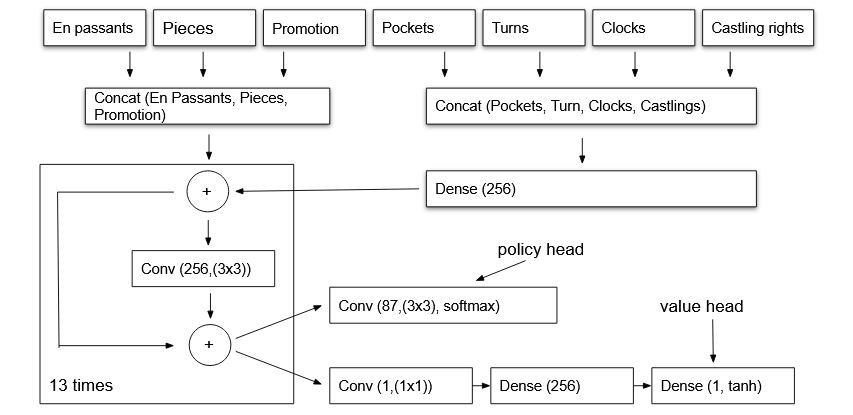
\includegraphics[width=0.9\textwidth]{resources/architecture}
	\caption{The architecture of the neural network. The number in the dense layer represents its number of neurons. In a convolutional layer it represents the amount of 8x8 boards, followed by its Kernel Size.}
	\label{img:architecture}
\end{figure*}
\\
The policy header is a convolutional layer with 87 filters that represent each possible action as a one-hot-vector.
Here we use a softmax activation function to get the probabilities of each move to played next (see \autoref{subsec:rep}).
The value head consists of a convolutional layer with a Kernel of 1x1 and one filter, which is then flattened.
This is followed by a dense layer of 256 Neurons followed by a dense layer with a tangent hyperbolic activation function for the value.
Output of the value head is number between -1 and 1, where 1 indicates a victory for the own team and -1 a defeat, respectively.
Unless otherwise mentioned we use a kernel of 3x3, a stride of one, zero padding, no dropout and ReLU activation functions.